\documentclass{beamer}
%Information
\title{AMC Introduction}
\titlegraphic{\hfill
\includegraphics[height=1cm]{orange.png}}
\institute{Youth STEM Academy}
\author{Erzhuo Wang}
\date{July 6,2024}
%Theme
\usetheme[block=fill, sectionpage=none]{metropolis}
\useoutertheme{infolines}
\useinnertheme{metropolis}
\setbeamertemplate{blocks}[rounded][shadow=false]
\setbeamertemplate{items}[ball]
\setbeamertemplate{sections/subsections in toc}[ball]
\setbeamertemplate{headline}{}
\logo{YSA}
\usecolortheme{custom}
%\usetheme{Madrid}
%\usetheme{Heverlee}

%Setting
\usepackage[UTF8,noindent]{ctexcap}
\theoremstyle{definition}
\newtheorem{defn}{Definition}[section]
\newtheorem{coro}[defn]{Corollary}
\newtheorem{theo}[defn]{Theorem}
\newtheorem{exer}[defn]{Exercise}
\newtheorem{rema}[defn]{Remark}
\newtheorem{lem}[defn]{Lemma}
\newtheorem{prop}[defn]{Proposition}
\newtheorem{nota}[defn]{Notation}
\newtheorem{exam}[defn]{Example}
\newtheorem{ques}[defn]{Question}

\newenvironment{prooff}{{\noindent\it\textcolor{cyan!40!black}{Proof}:}\,}{\par}
\newenvironment{proofff}{{\noindent\it\textcolor{cyan!40!black}{Proof of the lemma}:}\,}{\qed \par}
\newcommand{\bbrace}[1]{\left\{ #1 \right\} }
\newcommand{\bb}[1]{\mathbb{#1}}
\newcommand{\p}{^{\prime}}
\renewcommand{\mod}[1]{(\text{mod}\,#1)}
\newcommand{\blue}[1]{\textcolor{blue}{#1}}
\newcommand{\spec}[1]{\text{Spec}({#1})}
\newcommand{\rarr}[1]{\xrightarrow{#1}}
\newcommand{\larr}[1]{\xleftarrow{#1}}
\newcommand{\emptyy}{\underline{\quad}}
\newenvironment{enu}{\begin{enumerate}[(1)]}{\end{enumerate}}
%ctrl+点击文本返回代码  选中代码 ctrl+alt+j 为代码查找文本

\begin{document}
\begin{frame}
    \titlepage
\end{frame}
\section{Introduction}
\begin{frame}{Basic Information}
    The American Mathematics Competitions(AMC)
    is the preeminent math competition for students K-12.
    Today, over 300,000 students in 50 states and over 30 countries take the AMC to
    bolster their confidence and passion for math.
    \begin{figure}
        \centering
        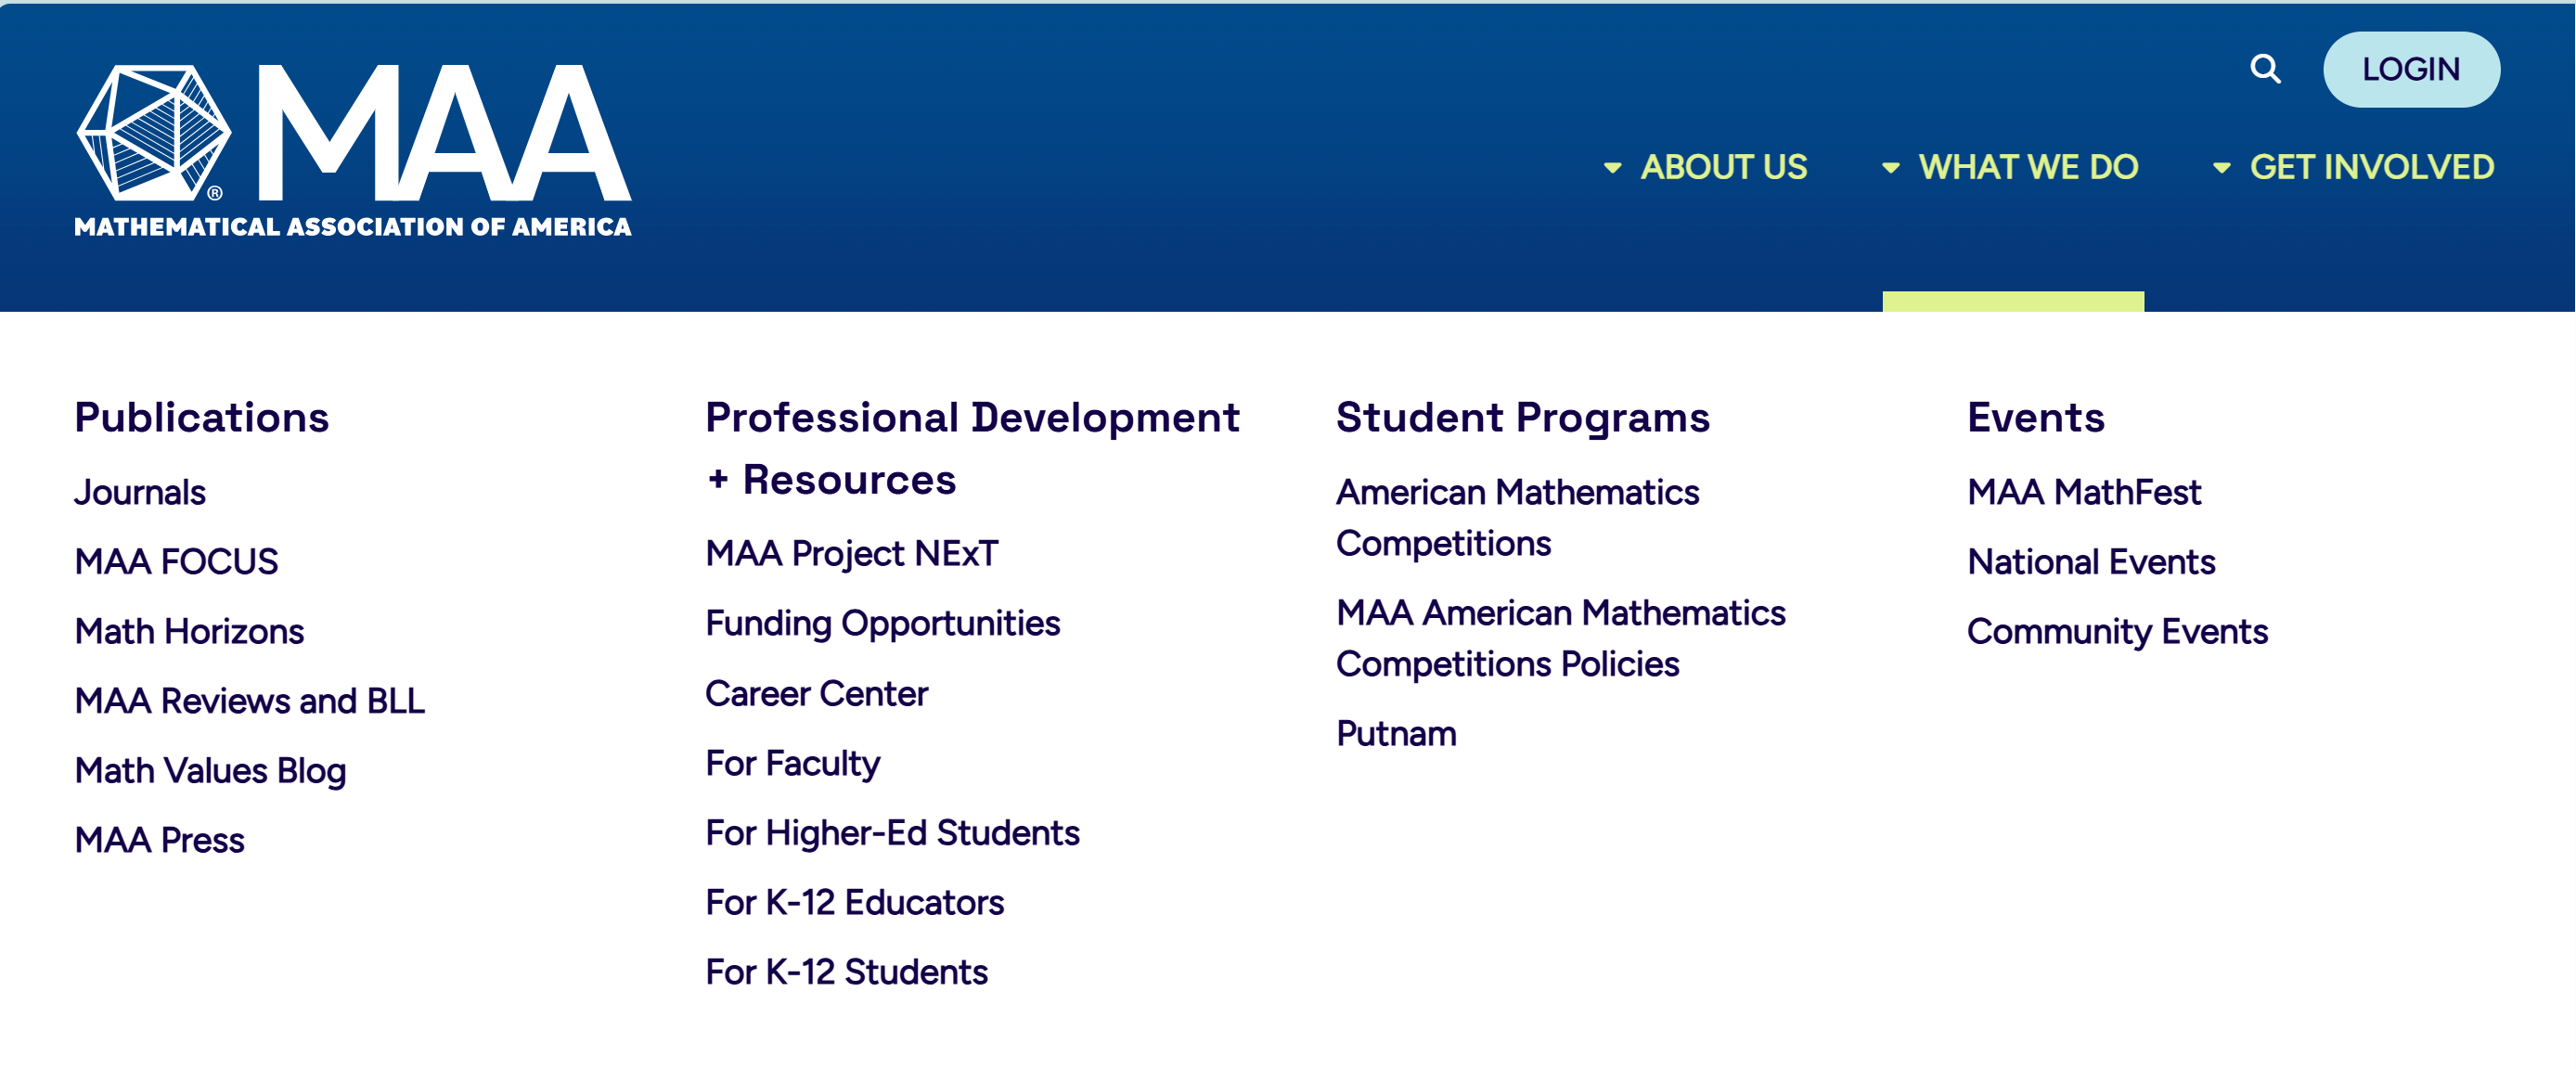
\includegraphics[width=0.8\textwidth]{MMA.png}
    \end{figure}
\end{frame}
\begin{frame}{Your Mathematical Journey: AMC to IMO}
    \begin{itemize}
        \item Begin your adventure with the AMC 8 for an introductory challenge or the
              AMC 10/12 for a chance to advance further in competitive mathematics.
        \item American Invitational Mathematics Examination (AIME):
              Excel in the AMC 10/12 to qualify for the AIME, a more challenging examination that tests your problem-solving prowess and mathematical ingenuity.
    \end{itemize}
\end{frame}
\begin{frame}{Your Mathematical Journey: AMC to IMO}
    \begin{itemize}
        \item USA Mathematical Olympiad and USA Junior Mathematical Olympiad (USAMO/USAJMO): Achieve high scores in the AIME and AMC 10/12 to earn an invitation to the USAMO or USAJMO, where the nation's top mathematical talents compete in proof-based problems.

        \item Mathematical Olympiad Program (MOP): Outstanding performance in the USAMO or USAJMO could lead to participation in the MOP, an intensive training camp designed to prepare the best young mathematicians for international competition.
    \end{itemize}
\end{frame}
% \begin{frame}{Compare with Chinese System}
%     \begin{table}
%         \centering
%         \begin{tabular}{c|c}
%             \hline
%             USA         & China                 \\
%             AMC 8/10/12 & 全国高中数学联赛预赛  \\
%             AIME        & 全国高中数学联赛      \\
%             USAMO       & 中国数学奥林匹格(CMO) \\
%             MOP         & 集训队选拔            \\
%             \hline
%         \end{tabular}
%     \end{table}
% \end{frame}
\begin{frame}{Rules}
    \begin{table}
        \centering
        \begin{tabular}{c|c|c|c}
            \hline
                             & AMC  8       & AMC 10       & AMC 12       \\
            Grade            & $\le 8$      & $\le 10$     & $\le 12$     \\
            Form             & 25 questions & 25 questions & 25 questions \\
            Time             & 40 minutes   & 75 minutes   & 75 minutes   \\
            Total Score      & 25           & 150          & 150          \\
            Scoring Criteria & (1,0,0)      & (6,1.5,0)    & (6,1.5,0)    \\
            \hline
        \end{tabular}
    \end{table}
    \begin{itemize}
        \item  $(x,y,z)$ means $x$ points for $1$ correct answer, $y$ points for $1$ blank answer and $z$ points for $1$ wrong answer.
    \end{itemize}

\end{frame}
\begin{frame}{规则}
    \begin{table}
        \centering
        \begin{tabular}{c|c|c|c}
            \hline
                     & AMC  8  & AMC 10    & AMC 12    \\
            年级     & $\le 8$ & $\le 10$  & $\le 12$  \\
            形式     & 25道题  & 25 道题   & 25 道题   \\
            事件     & 40 分钟 & 75  分钟  & 75  分钟  \\
            总分     & 25      & 150       & 150       \\
            判分方法 & (1,0,0) & (6,1.5,0) & (6,1.5,0) \\
            \hline
        \end{tabular}
    \end{table}
    \begin{itemize}
        \item  $(x,y,z)$为 对一个题$x$分,不填$y$分, 答错$z$分.
    \end{itemize}

\end{frame}
\begin{frame}{Range for AMC 8}
    \begin{itemize}
        \item Algebra: integer, rational number, real number, linear equation, inequality, number sequence, factorial, ratio.
        \item Combination: basic probability, Combinatorial number $\binom{n}{k}$
        \item Geometry: triangle, circle, rectangle, area, angle
        \item Number Theory: odd and even number,  divisor, GCD(greatest common divisor)
    \end{itemize}
\end{frame}

\begin{frame}{AMC 8考察范围}
    \begin{itemize}
        \item 代数: 解方程, 不等式, 数列, 阶乘, 比率.
        \item 组合: 概率, 组合数
        \item 几何: 三角形, 圆形, 矩形, 面积, 角度
        \item 数列: 奇数偶数, 整除, 最大公约数, 唯一因子分解
    \end{itemize}
\end{frame}
\begin{frame}{Algebra(代数)}
    \begin{itemize}
        \item 完全平方公式 $(x+y)^2=x^2+2xy+y^2$
        \item 平方差公式 $(x+y)(x-y)=x^2-y^2$
        \item 线性方程求解
              \begin{align*}
                  x+y=3 & \\
                  x-y=1 &
              \end{align*}
        \item 等差数列求和($1+3+5+7+9+\dots+101$是多少?)
        \item 等差数列求项数($1,4,7,11,\dots,100$共多少项?)
        \item 开根号$\sqrt{9}=?$
        \item 阶乘($5!=?$)
    \end{itemize}
\end{frame}
\begin{frame}{Number Theory(数论)}
    \begin{itemize}
        \item 整除(如何判断一个数能不能被3整除)
        \item 最大公约数, 最小公倍数(24和16最小公倍数是多少)
        \item 唯一因子分解, 勒让德公式
        \item 数论函数:除数个数函数,除数和函数$\sigma(n),\tau (n)$
    \end{itemize}
\end{frame}
\begin{frame}{Combinnation(组合)}
\begin{itemize}
    \item 组合数$\binom{n}{k}$
    \item 古典概型
    \item 条件概率$\mathbb{P}(A|B)$
\end{itemize}
\end{frame}
\begin{frame}{Geometry(几何)}
    \begin{itemize}
    \item 图形的面积, 周长
    \item 勾股定理($a^2+b^2=c^2$)
    \item 三角形相似,等腰直角三角形,$30,60,90$度的三角形
    \item 直线的方程,圆的方程
\end{itemize}
\end{frame}
\begin{frame}
    \begin{ques}
        How many odd three-digit integers have three distinct digits?

        有多少个奇三位数, 其个位十位百位各不相同?
        \pause
    \end{ques}
    \begin{prooff}
        If $n$ is odd, we have $5$ choices $1,3,5,7,9$ for its unit digits,

        Case 1: tens digit $=0$, there are $5\times 1\times 8$ numbers.

        Case 2: tens digit $\neq 0$, there are $5\times 8 \times 7$ numbers.
    \end{prooff}
\end{frame}
\begin{frame}{Handshakes}
    \begin{ques}
        Seven women and five men attend a party. At this party each man shakes hands with each other person once. Each woman shakes hands only with men.
        How many handshakes took place at the party?

        七女五男参加一个聚会。在这个聚会中, 每个男人会和其他人都握一次手, 每个女人只和男人握手, 请问这个聚会上会有多少次握手?
    \end{ques}
    \pause
    \begin{prooff}
        Firstly, let all the people shake hands with each other, then we get $\binom{12}{2}=66$ times handshakes.
        The total amount equals to $66$ minis the amount of handshakes between woman, that is $66-\binom{7}{2}=45$.
    \end{prooff}
\end{frame}
\begin{frame}{Solve this Euqation!}
    \begin{ques}[AMC 8, 2019-20]
        How many different real numbers $x$ satisfy the equation

        有多少不同的实数x满足这个方程
        \begin{equation*}
            (x^2-5)^2=16
        \end{equation*}
    \end{ques}
\end{frame}
\begin{frame}{Double Factorial(AMC 8, 2022-17)}
    If $n$ is an even positive integer, the double factorial notation $n$ !! represents the product of all the even integers from 2 to $n$. For example, $8!!=2 \cdot 4 \cdot 6 \cdot 8$. What is the units digit of the following sum?
    $$
        2!!+4!!+6!!+\cdots+2018!!+2020!!+2022!!
    $$
\end{frame}
\begin{frame}{Two Mountains(AMC 8, 2022-24)}
    如下图, 阴影部分面积为$183$, 求$h$.
    \begin{figure}
        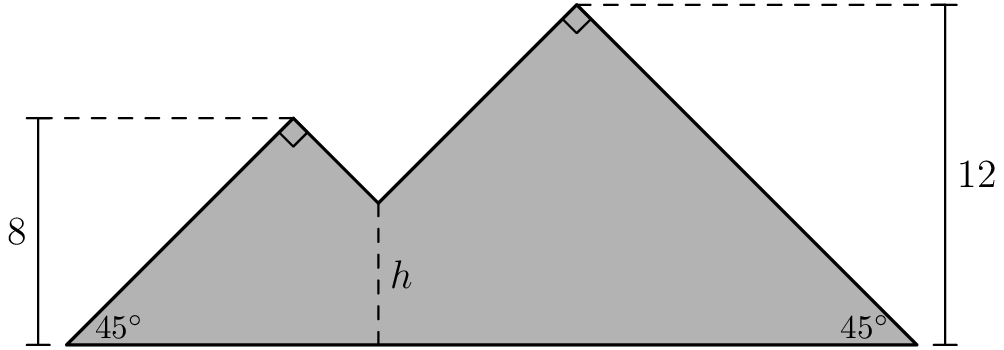
\includegraphics[height=0.4\textheight]{two mountains.png}
    \end{figure}
\end{frame}
\begin{frame}{双阶乘(AMC 8, 2022-17)}
    如果 $n$ 是一个偶数, $n!!$ 定义为从$2$到$n$所有偶数的乘积. 例如, $8!!=2 \cdot 4 \cdot 6 \cdot 8$. 请问如下求和的个位数?
    $$
        2!!+4!!+6!!+\cdots+2018!!+2020!!+2022!!
    $$
\end{frame}
\begin{frame}{Solution}
    Notice that once $n>8$, the units digit of $n$ !! will be 0 because there will be a factor of 10 . Thus, we only need to calculate the units digit of
    $$
        2!!+4!!+6!!+8!!=2+8+48+48 \times 8 =442
    $$
\end{frame}
\begin{frame}{Segment Coloring(AMC 8, 2024-23)}
    在平面直角坐标系上, 画一条从$(2000,3000)$到$(5000,8000)$的线段, 这条线段经过了多少个$1\times 1$的小方格(必须进入该方格的内部).
\end{frame}
\begin{frame}{Segment Coloring(AMC 8, 2024-23)}
    Rodrigo has a very large sheet of graph paper. First he draws a line segment connecting point $(0,4)$ to point $(2,0)$ and colors the 4 cells whose interiors intersect the segment, as shown below. Next Rodrigo draws a line segment connecting point $(2000,3000)$ to point $(5000,8000)$.
    How many cells will he color this time?
    \begin{figure}
        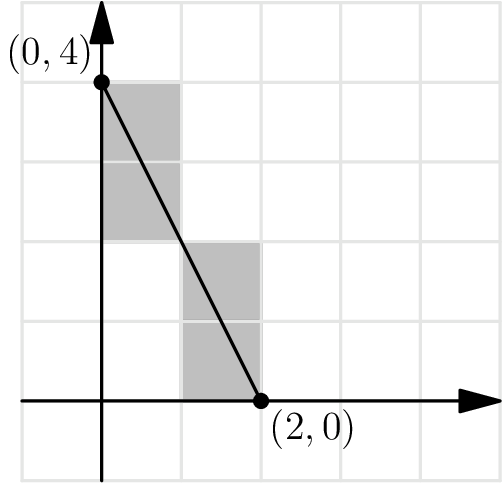
\includegraphics[height=0.5\textheight]{color the cell.png}
    \end{figure}
\end{frame}
\begin{frame}{Solution}
    Draw a line in the lattice which from $(2,3)$ to $(5,8)$, notice that the line crossed 7 blocks in this pattern.
    Such a pattern is repeated 1000 times between $(2000,3000)$ and $(5000,8000)$, then the answer is $7000$.
    \begin{figure}
        \centering
        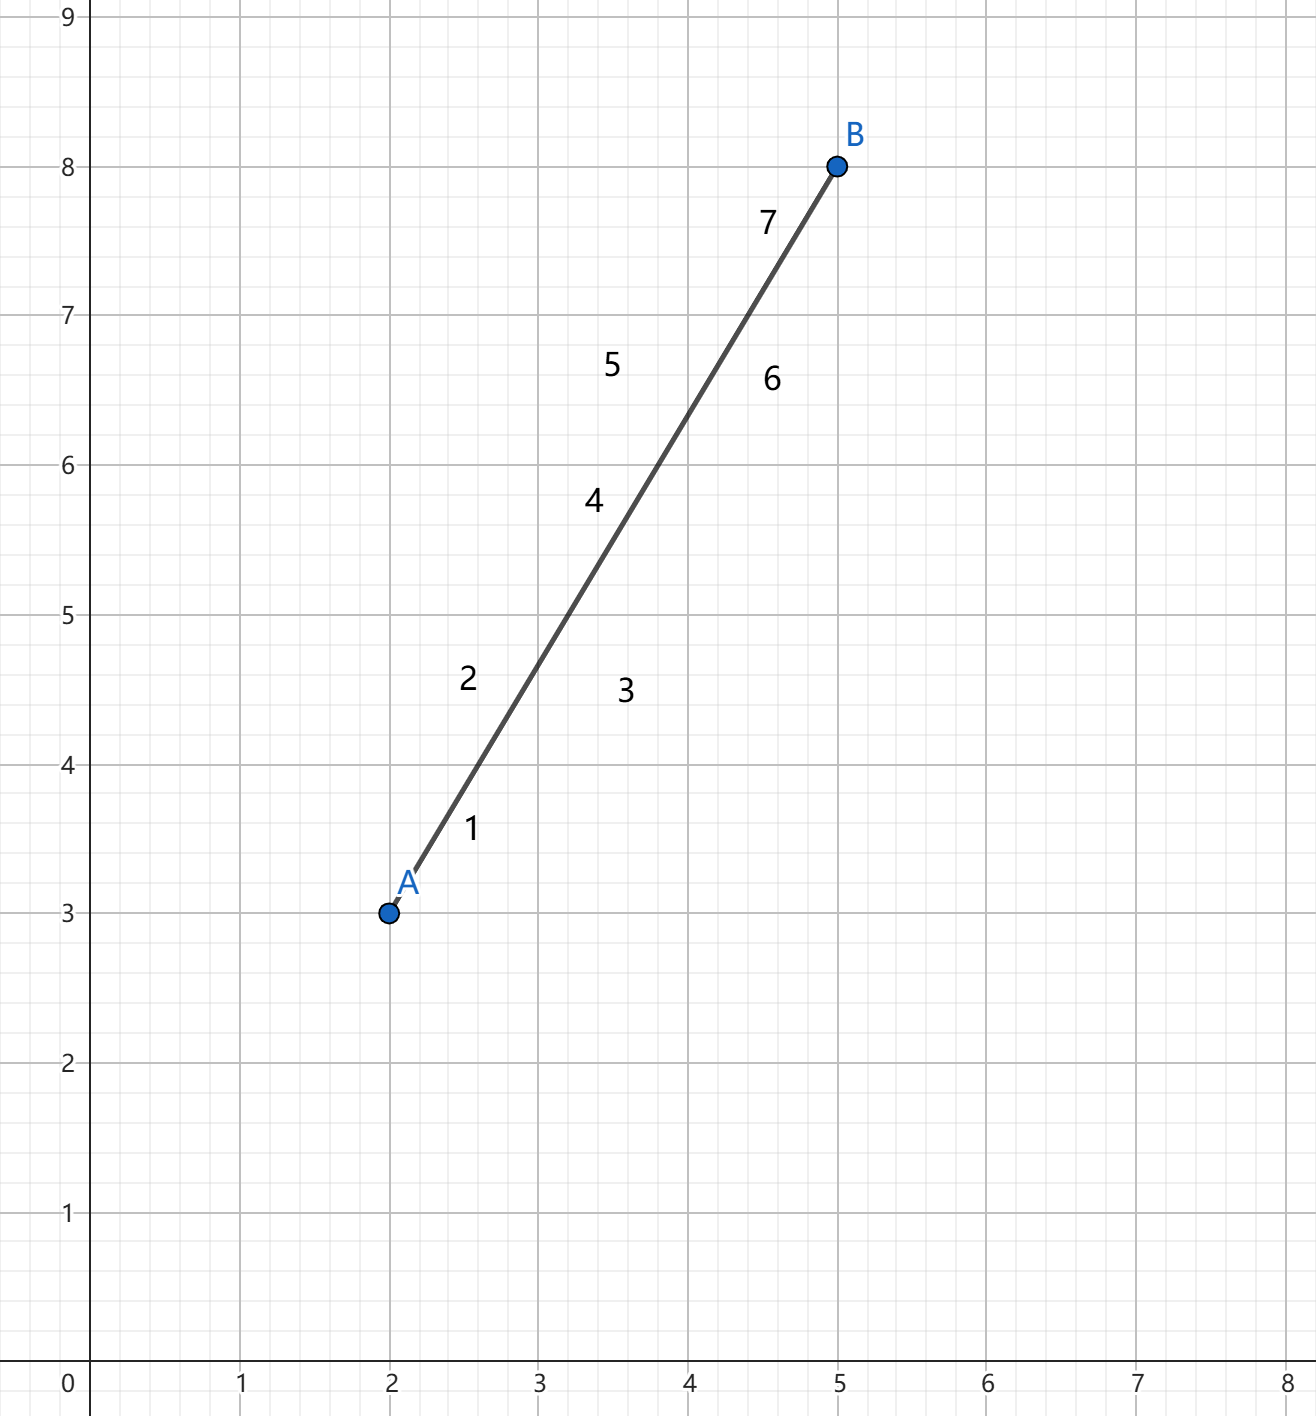
\includegraphics[height=0.5\textheight]{coloring.png}
    \end{figure}
\end{frame}
\begin{frame}{Jumping Cricket(AMC 8, 2022-25)}
    A cricket randomly hops between $4$ leaves,
    on each turn hopping to one of the other $3$ leaves with equal probability. After $4$ hops what is the probability that the cricket has returned to the leaf where it started?
    \begin{figure}
        \centering
        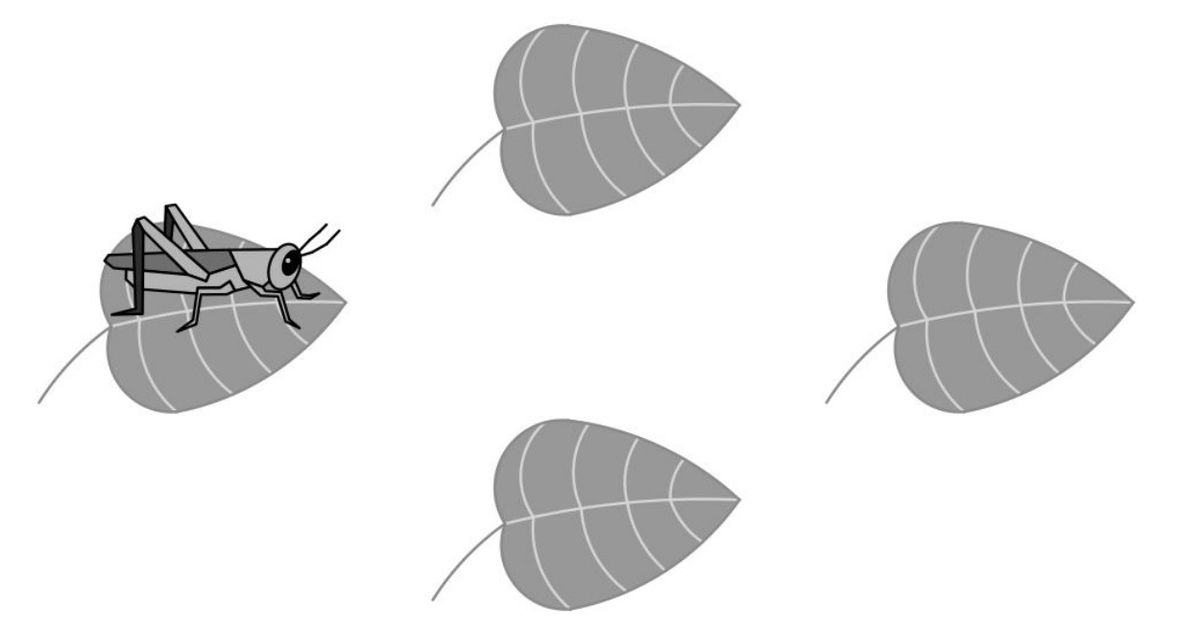
\includegraphics[width=0.5\textwidth]{AMC8-2022-25.jpg}
    \end{figure}
\end{frame}
\begin{frame}{跳跃的蟋蟀(AMC 8, 2022-25)}
    一个蟋蟀随意的在四片叶子上跳跃, 每次等概率得跳向其他三片叶子之一, 求蟋蟀跳四次后返回最初这片叶子的概率.
    \begin{figure}
        \centering
        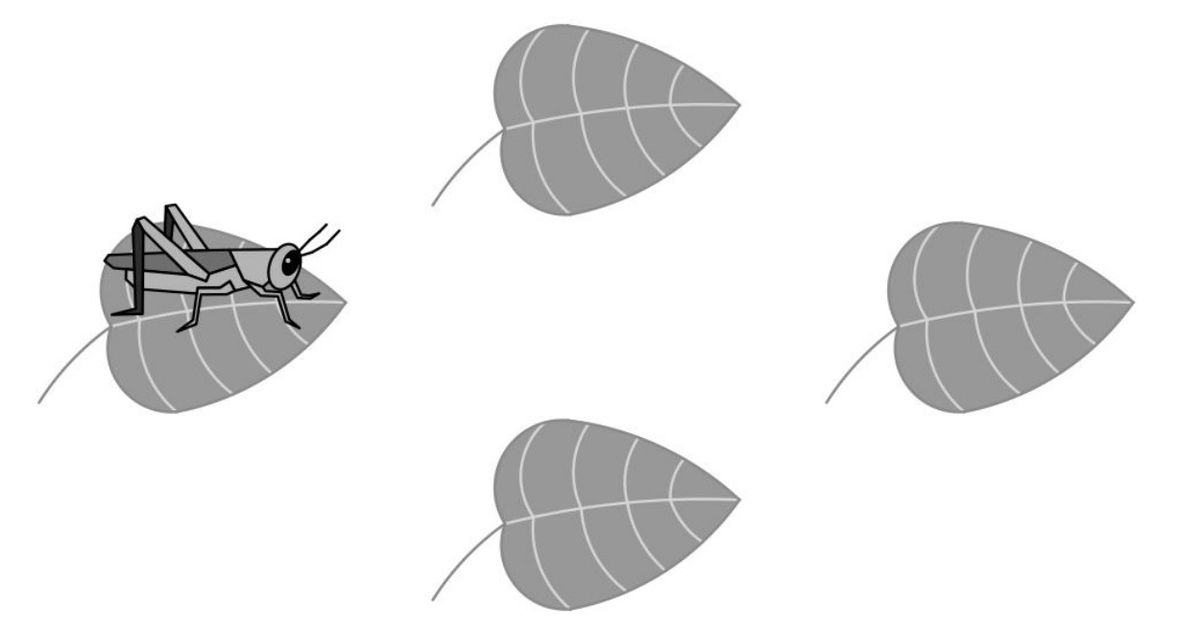
\includegraphics[width=0.5\textwidth]{AMC8-2022-25.jpg}
    \end{figure}
\end{frame}
\begin{frame}{Solution}

    Let $p_n$ be the probability that the cricket returns to the leaf after $n$ times jumping. $q_n$ be the
    probability that the cricket doesn't retrun to the leaf.
    We have the recursion equations
    \begin{equation*}
        p_n+q_n=1
    \end{equation*}
    and
    \begin{equation*}
        p_n=\frac{1}{3}q_{n-1}
    \end{equation*}
    Hence
    \begin{equation*}
        p_1=0,p_2=\frac{1}{3},p_3=\frac{2}{9},p_4=\frac{7}{27}
    \end{equation*}
\end{frame}
\end{document}